\documentclass[12pt]{article} % use larger type; default would be 10pt

%packages
\usepackage[utf8]{inputenc} % set input encoding (not needed with XeLaTeX)
\usepackage{fancyhdr}
\usepackage{float}
\usepackage{geometry}
\usepackage{ulem}
\usepackage{soul}
\usepackage{color}
\usepackage{graphicx}
\usepackage{hyperref}
\usepackage{array}
\usepackage{caption}
\usepackage{titling}
\usepackage{enumerate} 
\usepackage[dvipsnames]{xcolor}
\usepackage{amsmath}
\usepackage{amssymb}
\usepackage[compact]{titlesec}


 %put box around figure captions
\makeatletter
\long\def\@makecaption#1#2{%
  \vskip\abovecaptionskip
  \sbox\@tempboxa{\fbox{#1: #2}}%
  \ifdim \wd\@tempboxa >\hsize
    \fbox{\parbox{\dimexpr\linewidth-2\fboxsep-2\fboxrule}{#1: #2}}\par
  \else
    \global \@minipagefalse
    \hb@xt@\hsize{\hfil\box\@tempboxa\hfil}%
  \fi
  \vskip\belowcaptionskip}
\makeatother

%reduce space between sections
\titlespacing{\section}{0pt}{*1}{*0}
\titlespacing{\subsection}{0pt}{*1}{*0}
\titlespacing{\subsubsection}{0pt}{*0}{*0}


%no indent and modify distance between paragraphs
\setlength\parindent{0pt}
\setlength\parskip{12pt}

%set margins and line spacing
\geometry{margin=1in}
\linespread{1.2}
\geometry{letterpaper}

%math operators
\DeclareMathOperator{\E}{\mathbb{E}}

%set up header and page numbering
\pagestyle{fancy}
\lhead{Scientific Appendix}
\rhead{Timothy Liu}
\pagenumbering{arabic}

\hypersetup{  %set up url
    colorlinks=true,
    linkcolor=blue,
    filecolor=magenta,      
    urlcolor=cyan,
}



\title{PyCli Modeling}
\author{Timothy Liu}

\begin{document}

\maketitle

\tableofcontents

\newpage

% Introduction
\section{Introduction}
PyCli uses a discrete energy balance model for modeling temperatures across the globe. The planet is discretized into a grid with the size of each grid cell a fixed number of degrees latitude and longitude. Since the number of cells at each latitude band is fixed, the cells closer to the poles are smaller than the cells at the equator.

This document describes the PyCli backend climate model. Several versions of the model are implemented in C++ in the \textbf{src} folder. This document focuses on the physics of the model, and does not elaborate on how it is actually implemented.

The energy balance models described in \hyperref[sec:model]{Section 2} balances the incoming solar radiation with outgoing radiation to calculate the surface temperature. The incoming radiation is determined by the latitude of the cell, and the calculations for finding the incoming radiation for each cell is described in \hyperref[sec:radiation]{Section 3}.  The surface is treated as having one of several types: ocean, land, and ice. Each of the surface types has an associated albedo, and more details can be found in \hyperref[sec:surface]{Section 3}. The atmosphere is the most complex piece of the model, and is described in \hyperref[sec:atmos]{Section 4}. The greenhouse gas is calculated by considering the infrared transmissivity of the atmosphere, combined with the adding radiation forcing of carbon dioxide. Finally, a crude model for heat distribution between cells based on a 2D convolution is described in \hyperref[sec:heatflow]{Section 5}.

% Two Layer Energy Balance Model
\newpage
\section{Energy Balance Model}
\label{sec:model}

\subsection{Two Layer Energy Balance Model}

PyCli uses a fairly simple variation of the two layer energy balance model to calculate temperatures at each element in the grid. The same set of calculations are performed for each grid element, with the albedo and incoming solar radiation dependent on each individual element. The energy balance model is illustrated in Figure~\ref{fig:2layer}. Note that the PyCli model uses a variation of the two layer model described in this subsection - the modification is described in the next section.

\begin{figure}[H]
	\makebox[\textwidth][c]{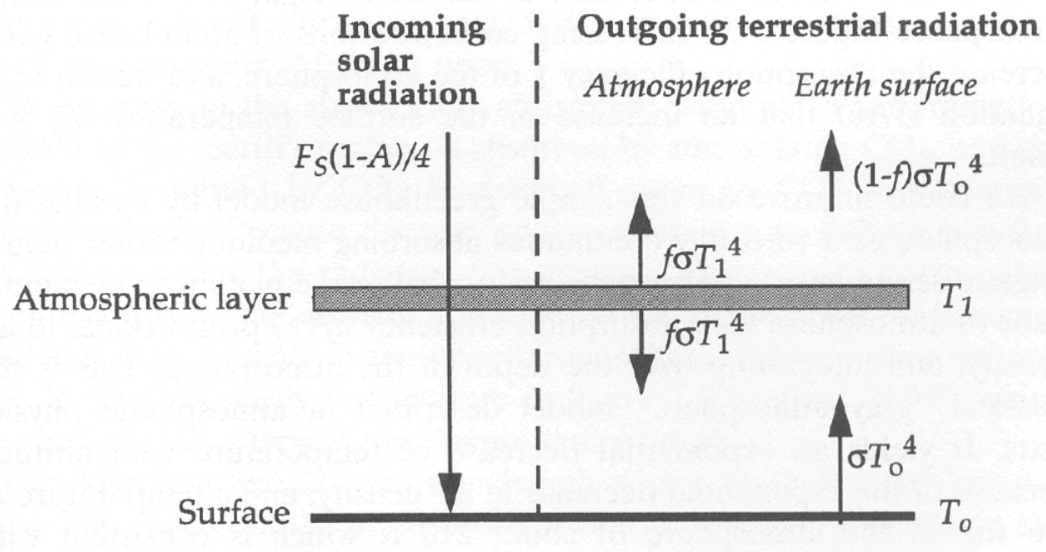
\includegraphics[width=4in]{2layer.png}}
	\caption{Two layer energy balance model. Note that the radiation forcing from carbon dioxide is not included in the model.}
	\label{fig:2layer}
\end{figure}

The atmosphere is modeled as a single layer that is transparent to incoming solar radiation. The solar radiation is partly reflected (not illustrated) and the remaining absorbed solar radiation is re-emitted as infrared radiation. The emission from the surface is modeled by Planck's law as blackbody radiation. The atmosphere is partially opaque to the outgoing infrared radiation. The absorbed radiation is then re-emitted, with half of the radiation emitted into space and the other half emitted back to the surface.

The energy balance at the top of the atmosphere is described by:

$$E_{in}(1-A)  = (1-f) \sigma T_0^4 + f \sigma T_1^4$$

where $f$ is the fraction of infrared energy absorbed by the atmosphere, $A$ is the albedo of the surface, and $E_{in}$ is the average power per unit area of the surface. This equation balances the incoming solar radiation that is not reflected with the outgoing infrared energy emitted by the surface that passes through the atmosphere and the infrared energy emitted by the atmosphere, respectively. Note that in Figure~\ref{fig:2layer} the incoming energy is expressed as $\frac{1}{4}$ the sun's radiation while in the equation we have simplified this to the average power across all times of day.

The energy balance at the atmosphere layer is: 
$$2f\sigma T_1^4 = f\sigma T_o^4$$

which balances the infrared energy emitted by the atmosphere with the energy emitted by the surface absorbed by the atmosphere.

Combining these equations gives us equations for the temperature at the surface and the atmosphere:

$$T_0 = \bigg( \frac{(1-A)E_{in}}{\sigma(1-\frac{f}{2})}  \bigg)^{\frac{1}{4}}$$

$$T_1 =  2^{-\frac{1}{4}} T_0 $$

\subsection{Modified Two Layer Energy Balance Model}

The two layer energy balance model requires a fraction $f$ that describes the fraction of infrared radiation absorbed by the atmosphere. Specifically, the model demands an expression for $f$ in terms of the concentrations of different greenhouse gases, primarily carbon dioxide, water vapor, and ozone. However, computing this function is non-trivial, and the PyCli model makes a simplification that divides greenhouse gases into two categories.

Water vapor and ozone are considered ``constant greenhouse gases" whose concentration is fixed. The value of $f$ for just these two constant greenhouse gases is described in \hyperref[sec:atmos]{Section 4}. Carbon dioxide is considered a ``varying greenhouse gas" whose concentration can be changed and is an input to the model. Rather than calculating carbon dioxides contribution to $f$, the PyCli model uses the following empirical equation from Myhre et al. (1998):

$$ E_{CO_2} = 5.35 W m^{-2} ln \frac{[CO_2]}{280ppm}$$

The contribution from carbon dioxide is directly calculated using this formula and added to the downward emitted from the atmosphere towards the ground.


The energy balance at the top of the atmosphere remains the same:

$$ E_{in}(1-A)  = (1-f) \sigma T_0^4 + f \sigma T_1^4$$

While the energy balance between the surface and the atmosphere becomes:

The energy balance at the atmosphere layer is: 
$$2f\sigma T_1^4 + E_{CO_2} = f\sigma T_o^4$$

Combining these two equations again gives us expressions for the surface temperature:

$$\boxed{T_0 = \bigg[ \bigg((1-A)E_{in} + \frac{E_{CO_2}}{2}\bigg)\bigg(\frac{1}{\sigma(1-\frac{f}{2})}\bigg)\bigg] ^{\frac{1}{4}}}$$

% Incoming Solar Radiation
\newpage
\section{Incoming Solar Radiation}
\label{sec:radiation}

The solar radiation falling on the entire Earth is:

$$E_{total} = E_{sun} \pi r_{Earth}^2$$

Consider the Earth as a flat disc perpendicular to the direction of the sun. The sunlight falling on a horizontal strip is:

$$E_{strip} = 2 E_{sun} \int_{x_0}^{x_f} \sqrt{r_{E}^2 - x^2} dx$$


where $x_0$ and $x_f$ are the distances from the equator of the bottom and top of the strip. Integrating to the get the closed form:

$$E_{strip} = 2 E_{sun} \frac{1}{2} x \sqrt{r_{E}^2 - x^2} - \frac{1}{2} r_{E}^2 \tan^{-1}\bigg({\frac{x \sqrt{r_{E}^2 - x^2}}{x^2 - r_{E}^2 }}\bigg)\bigg]_{x_0}^{x_f}$$

$$E_{strip} = W_{sun} x \sqrt{r_{E}^2 - x^2} -  r_{E}^2 \tan^{-1}\bigg({\frac{x \sqrt{r_{E}^2 - x^2}}{x^2 - r_{E}^2 }}\bigg)\bigg]_{x_0}^{x_f}$$

However, the boundaries between the cells are defined by lines of latitude rather than as a distance from the equator of a flat disc. The substitution: 

$$x = r_{E} sin(\theta) $$

where $\theta$ is the line of latitude, is used to convert between $x$ and the line of latitude $\theta$. The incoming solar flux per
unit area along this strip is the above result divided by the surface area of the strip on a 3D sphere:

$$A_{strip} = \int_{\theta_{0}}^{\theta_{f}} 2 \pi r_{E} \cos{\theta} r d\theta $$

where $2 \pi r_{E} \cos{\theta}$ is the circumference of the earth at a certain latitude and $r d\theta$ is the north-south distance of a differential along the surface of the earth. This can be simplified to:

$$A_{strip} =  2 \pi r_{E}^2 \sin{\theta}\bigg]_{x_0}^{x_f} $$

The average solar flux falling on a cell in a strip bound by $\theta_0$ and $\theta_f$ is:

$$E_{in} = \frac{E_{strip}}{A_{strip}}$$

$$\boxed{E_{in} = E_{sun}\frac{x \sqrt{r_{E}^2 - x^2} -  r_{E}^2 \tan^{-1}\bigg({\frac{x \sqrt{r_{E}^2 - x^2}}{x^2 - r_{E}^2 }}\bigg)\bigg]_{r_{E}\sin(\theta_0)}^{r_{E}\sin(\theta_f)}}{2 \pi r_{E}^2 \sin{\theta}]_{\theta_0}^{\theta^f}}}$$

Please note that the argument of the $\tan^{-1}$ approaches $-\infty$ as $x$ approaches $r_{E}$. The limit of $\tan^{-1}$ approaches $-\frac{\pi}{2}$ so when $x = r_{E}$ the numerator reduces to:

$$x \sqrt{r_{E}^2 - x^2} -  r_{E}^2 \tan^{-1}(-\infty)$$

$$0 -  r_{E}^2 (-\frac{\pi}{2})$$

$$\frac{r_{E}^2 \pi}{2}$$

% Surface
\newpage
\section{Surface}
\label{sec:surface}

In the PyCli model, the surface can be one of three types: land, sea, and ice. Each of the three types has a different albedo:

\begin{center}
\begin{tabular}{|m{4 cm}| m{2 cm}|} \hline
\textbf{Type} & \textbf{Albedo} \\ \hline
Land & 0.2\\ \hline
Sea & 0.06\\ \hline
Ice & 0.6\\ \hline
\end{tabular}
\end{center}

Regardless of the calculated temperature, the surface types do not change.


% Atmosphere
\newpage
\section{Atmosphere}
\label{sec:atmos}

The PyCli atmosphere is uniform around the globe. It is modeled as a single layer that is transparent to incoming visible light but partially absorbs outgoing infrared light. The subsections below describe how the fraction of infrared energy absorbed by the atmosphere $f$ is calculated, which is then input into the energy balance model.

Only some gases are considered. Nitrogen and oxygen are both included in the model, but are considered inert. There is a fixed amount of ozone and water vapor, which both contribute a constant amount to infrared absorption. Finally, the level of carbon dioxide can be changed by the user. Carbon dioxide does not contribute to the infrared absorption of the atmosphere; instead, the radiative forcing from $CO_2$ is directly added to the energy balance model.


\subsection{Infrared Absorption}

Some of the infrared energy radiated by the Earth's surface is absorbed by the atmosphere. The presence of greenhouse gases contributes to how much of the infrared energy is absorbed.

The energy emitted by the Earth is approximated by blackbody radiation described by Planck's law:

\begin{figure}[H]
	\makebox[\textwidth][c]{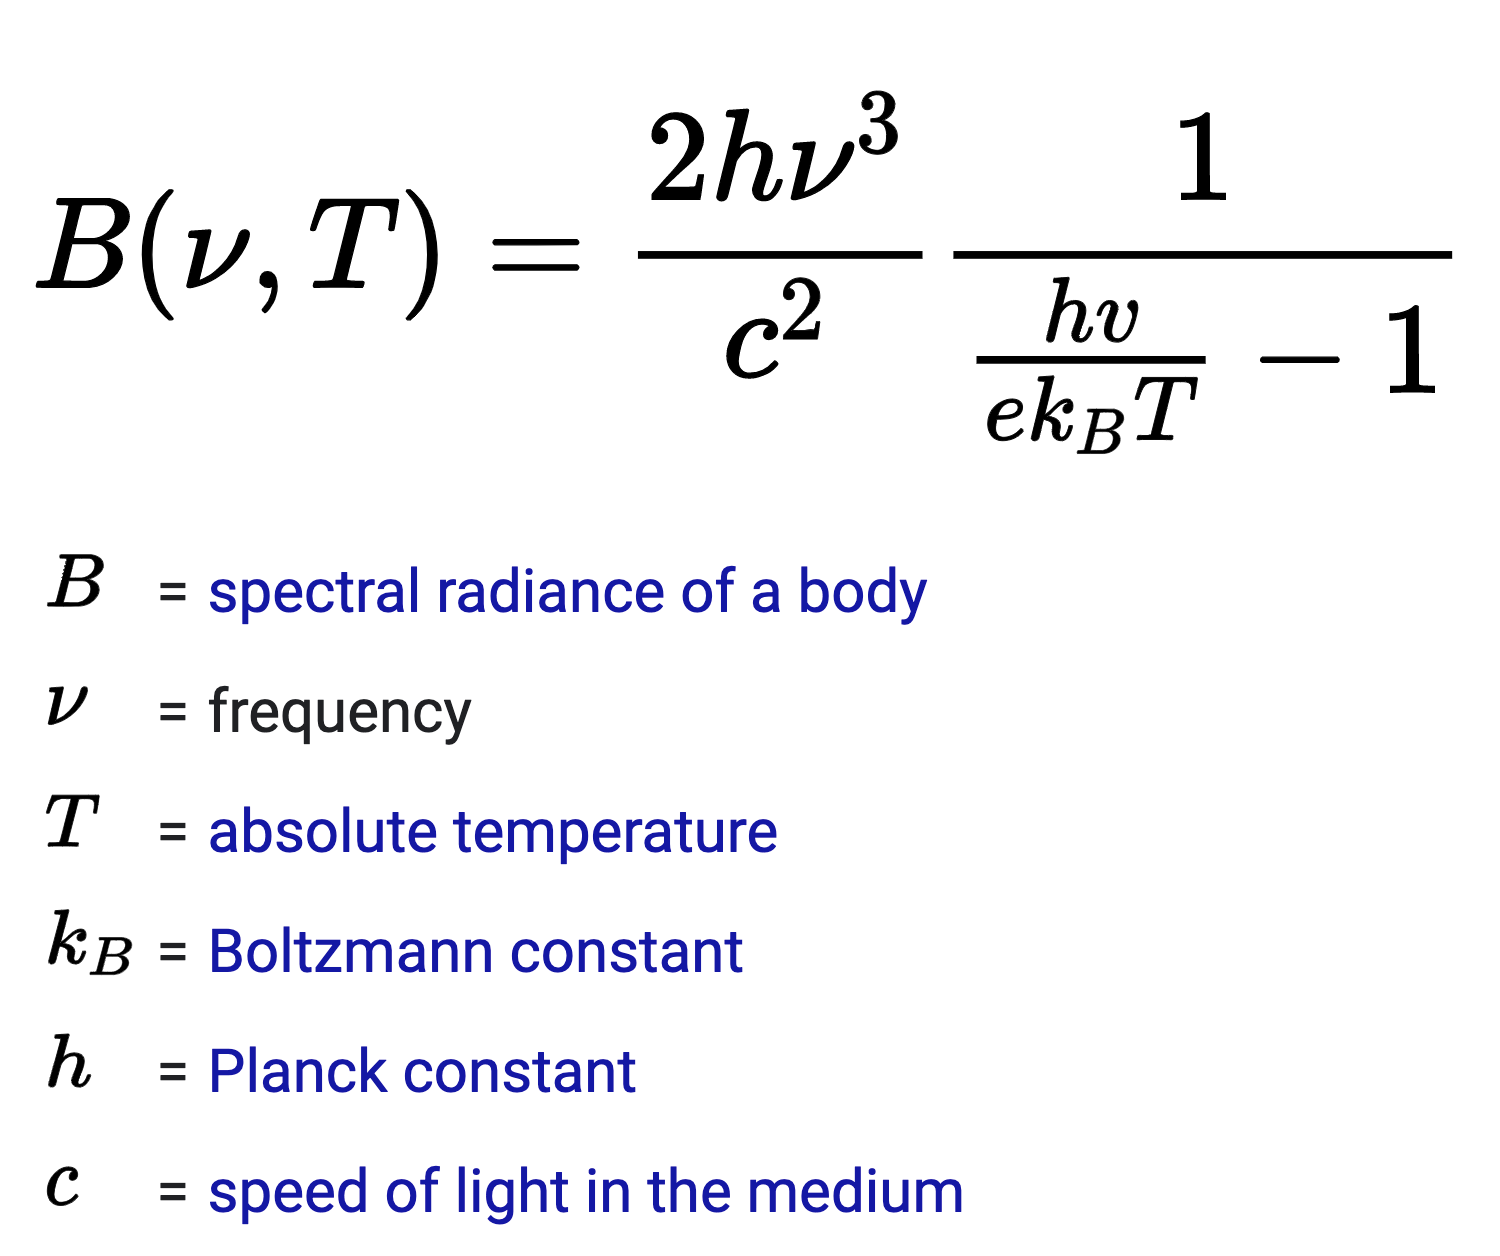
\includegraphics[width=3in]{planck_law.png}}
	\caption{Spectral radiance as a function of wavelength and temperature.}
	\label{fig:planck_law}
\end{figure}

Figure~\ref{fig:planck} illustrates Planck's law at different temperatures close to Earth's surface temperature. The energy absorbed by the atmosphere can be calculated by integrating over the absorption spectrum of greenhouse gases. 

\begin{figure}[H]
	\makebox[\textwidth][c]{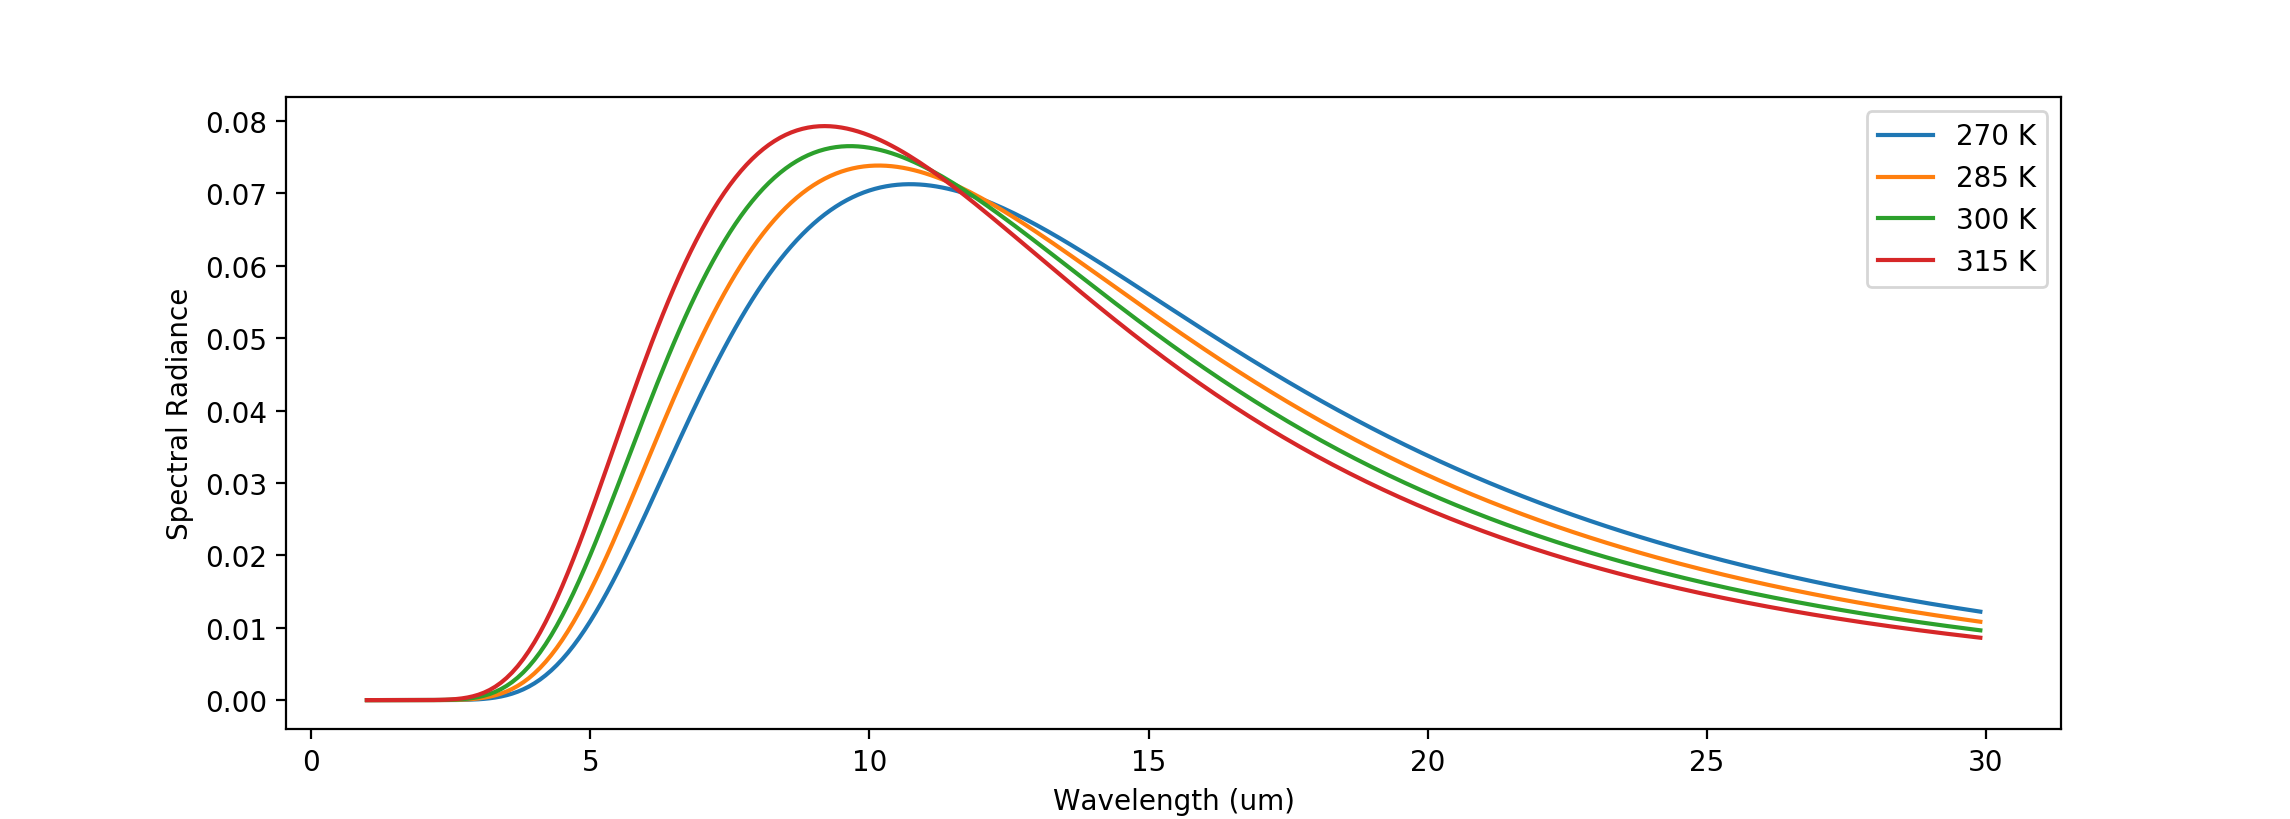
\includegraphics[width=5in]{planck.png}}
	\caption{Spectral radiance as a function of wavelength and temperature.}
	\label{fig:planck}
\end{figure}

Assume we have a function $A(\lambda)$ that describes the fraction of energy absorbed by the atmosphere at different frequencies. The total fraction of energy absorbed by the atmosphere is then:

$$\frac{\int_{\lambda_0}^{\lambda_f} A(\lambda) B(\lambda, T) d\lambda}{\int_{\lambda_0}^{\lambda_f} B(\lambda, T) d\lambda }$$

Note that we've reformulated Planck's law in terms of wavelength instead of frequency. However, note that the expression for $B$ is dependent on surface temperature, which is the value we're ultimately trying to solve for! As an approximation, we choose a temperature of 288 K, which is close to Earth's average surface temperature, as an input into Planck's law to create the distribution of emitted energy.

\subsection{Creating an expression for $A(\lambda)$}

In the previous step we assumed we had an expression for $A(\lambda)$ to calculate the fraction of infrared energy absorbed by the atmosphere. This subsection describes how this expression is actually derived. The PyCli model considers two constant greenhouse gases that contribute to $f$, the fraction of light absorbed by the atmosphere: ozone and water vapor.  Figure~\ref{fig:absorb} shows how much IR these two gases absorb.

\begin{figure}[H]
	\makebox[\textwidth][c]{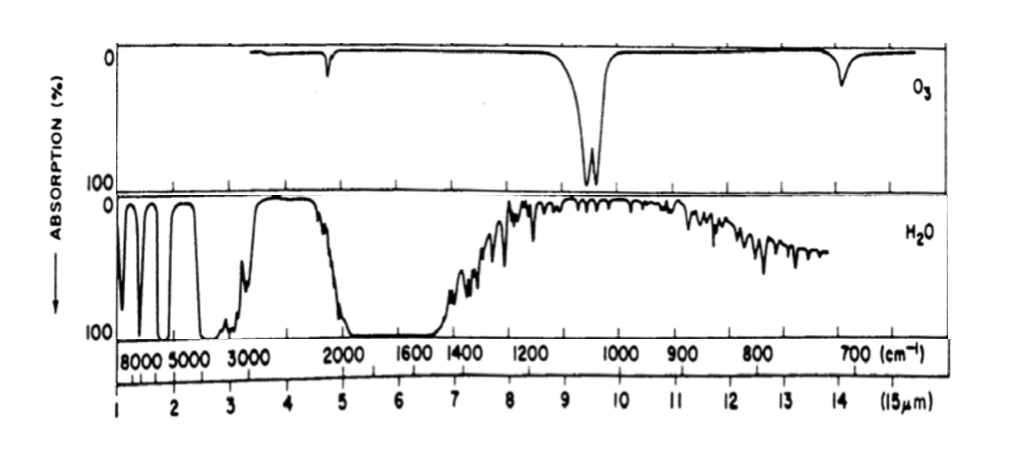
\includegraphics[width=5in]{absorb.png}}
	\caption{Fraction of IR absorbed by ozone and water vapor as a function of wavelength. Note that the y-axis is inverted.}
	\label{fig:absorb}
\end{figure}

The IR light that is not absorbed is transmitted. The combined transmittance of multiple gases is the product of the transmittance of the individual species. By combining the absorption of the constant greenhouse gases, Figure~\ref{fig:combine_absorb} gives the absorption of the atmosphere as a function of wavelength, $A(\lambda)$.

\begin{figure}[H]
	\makebox[\textwidth][c]{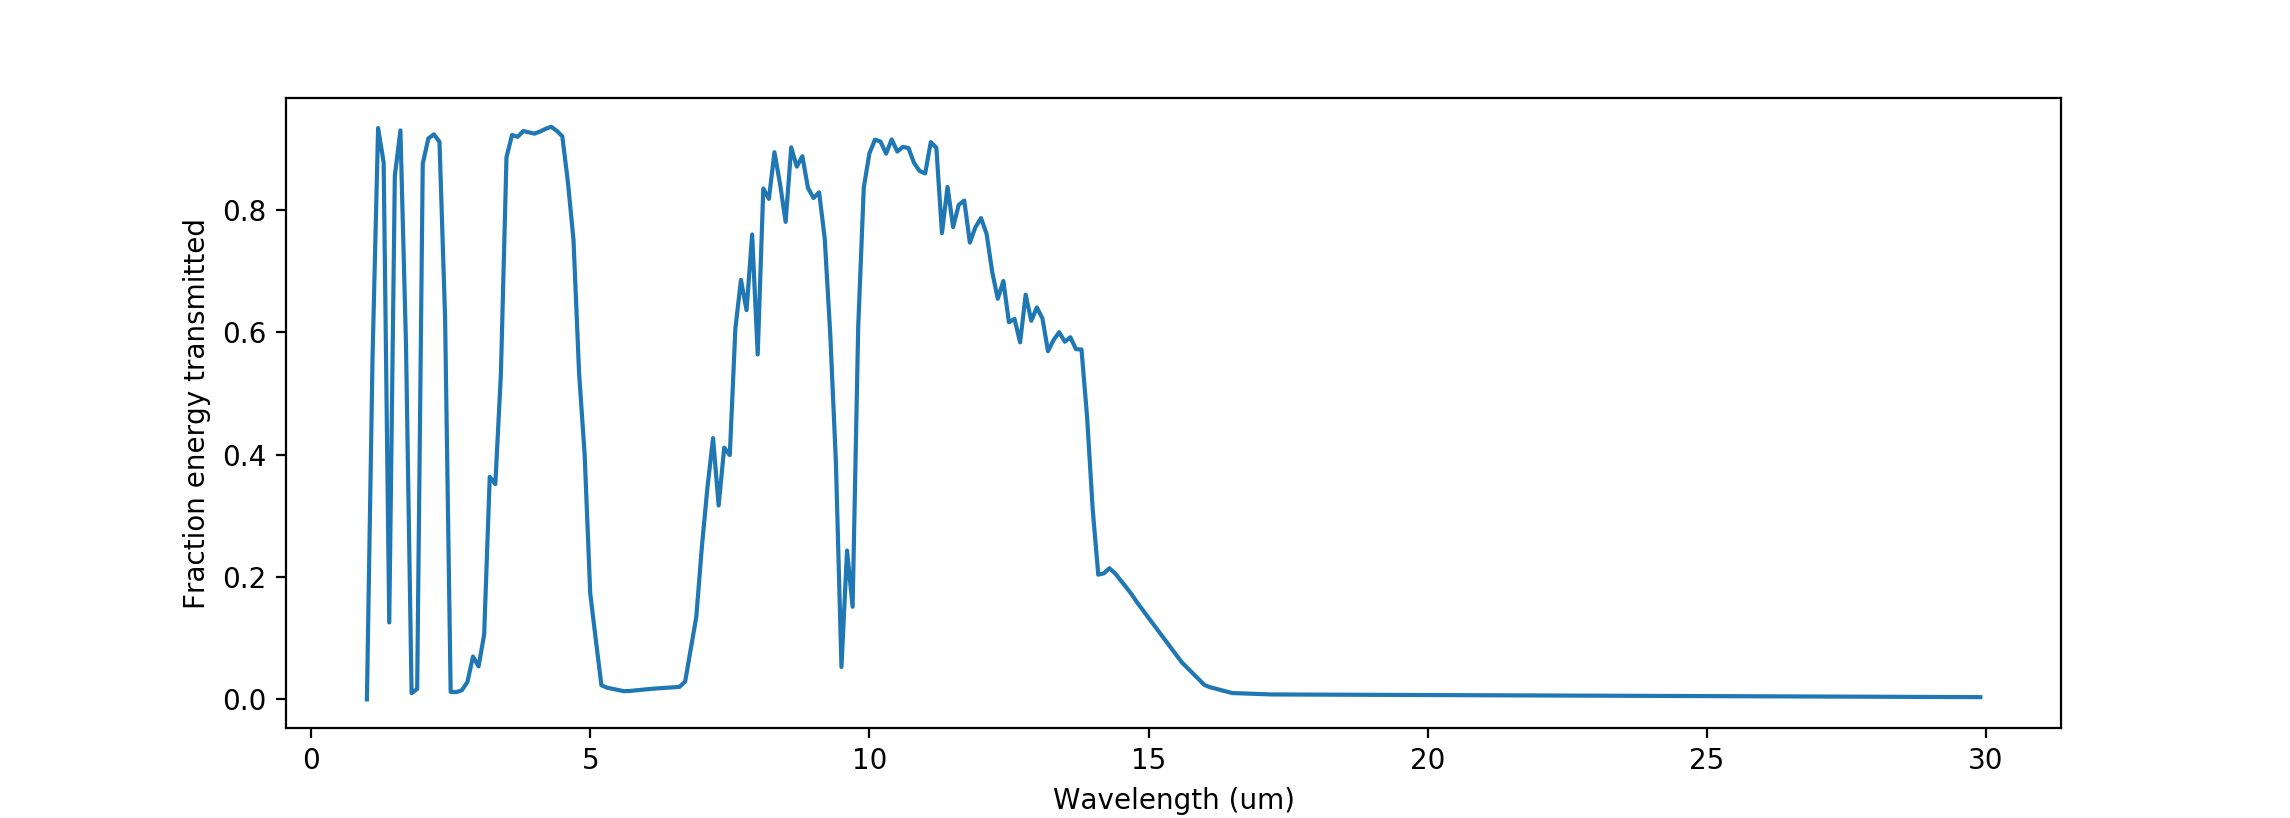
\includegraphics[width=5in]{combine_absorb.png}}
	\caption{Fraction of IR absorbed by the constant greenhouse gases in PyCli as a function of wavelength.}
	\label{fig:combine_absorb}
\end{figure}

\subsection{Value of $f$}
The value of $f$ can be calculated by integrating the fraction of energy absorbed multiplied by the fraction of energy emitted as a function of wavelength. This is the same as integrating the product of Figure~\ref{fig:combine_absorb} and Figure~\ref{fig:planck}. The limits of integration is the range of wavelengths where a significant amount of energy is emitted. 

$$\frac{\int_{\lambda_0}^{\lambda_f} A(\lambda) B(\lambda, T) d\lambda}{\int_{\lambda_0}^{\lambda_f} B(\lambda, T) d\lambda }$$

Integrating numerically gives a final value for $f$ of \textbf{0.665} with $\lambda_0 = 1um$ and $\lambda_f = 40 um$.

%heat flow
\newpage
\section{Heat Flow}
\label{sec:heatflow}

A simple model is used to simulate how heat moves between adjacent squares. After the temperatures are calculated using the energy balance model, a 2D convolution is applied over the surface. The convolution uses a Gaussian kernel with a width that is equal to 10\% of the circumference of the planet. For example, if the surface is 900 squares wide then the kernel has 90 elements.

The grid is treated as if it's wrapped around a cylinder in the convolution. Grid elements on the far right edge of the grid are considered to be adjacent to the elements on the far left edge. The top and bottom (north and south) edges do not wrap over the poles; instead, the top and bottom most boundary values are repeated in the convolution.

%Appendix 1
\newpage
\section{Appendix 1: Variable names}

\begin{center}
\begin{tabular}{|m{2 cm}| m{6 cm}| m{6 cm}|} \hline
\textbf{Variable} & \textbf{Description} & \textbf{Units}\\ \hline
$E_in$ & Incoming solar radiation & watts per square meter\\ \hline
$A$ & Albedo & fraction\\ \hline
$f$  & fraction of outgoing infrared radiation absorbed by atmosphere & fraction \\ \hline
\end{tabular}
\end{center}


% references
\newpage
\section{References}
\label{sec:references}



\end{document}
